\section{Electrodiffusion in the extracellular space}
\label{sec:eldiff}
In the standard VC theory presented in Chapter \ref{sec:VC_theory}), we assumed that extracellular currents, and thus extracellular potentials, are exclusively due to ohmic drift. However, when ion concentrations are present in the extracellular space, there will also be diffusive currents present, which can evoke so called diffusion potentials. 

In this chapter, we will introduce a more general, electrodiffusive theory for extracellular dynamics, which accounts effects of ionic diffusion as well as ohmic drift. However, before we present the electrodiffusive theory, we will try to get an intuition of how diffusion potentials arise.

\subsection{What is a diffusion potential?}
To get a qualitative understanding of what a diffusion potential is, let us consider a simple two-compartment system with two ionic solutions interacting at a junction  (Fig. \ref{fig:diffpot}). We assume that we in one compartment (the left) have a high concentration of NaCl, and in the other compartment (the right) have a lower concentration of NaCl (Fig. \ref{fig:diffpot}A). Initially, both compartments are electroneutral, i.e., they contain equal amounts of Na$^+$ and Cl$^-$. As there are no electrical forces present, the initial system dynamics will be driven exclusively by diffusion. 

\begin{figure}[!ht]
\begin{center}
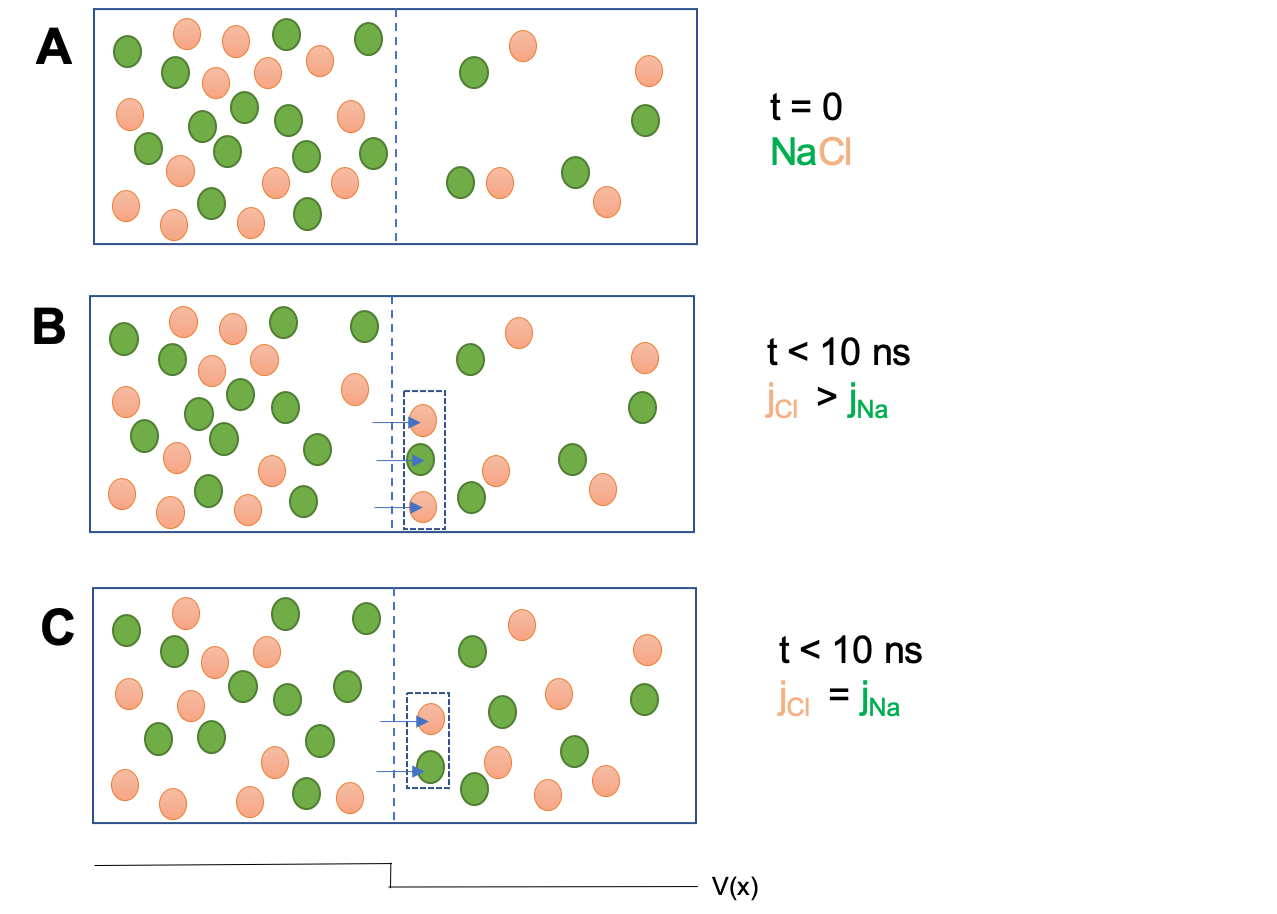
\includegraphics[width=0.8\textwidth]{Figures/Diffusionpot.png}
\end{center}
\caption{\textbf{Diffusion potential at the junction between two ionic solutions}. ({\bf A}) Initial condition with high concentration NaCl in the left compartment and low concentration NaCl in the right compartment. ({\bf B}) Since $D_{Cl} > D_{Na}$, we initially expect the flux of Cl$^-$ to be higher than the flux of Na$^+$. ({\bf C}) The net charge transfer in ({\bf B}) will give rise to a potential difference $\phi_d$ between the two compartments, which will prevent further charge accumulation. }
\label{fig:diffpot}
\end{figure}

Without solving any equations, we intuitively realize that initially, both Na$^+$ and Cl$^-$ will diffuse towards the low-concentration compartment on the right-hand-side. The diffusion speed for the various ions will be proportional to their respective diffusion constants, which in dilute solutions have the values given in Table \ref{tab:diffconsts}). As the Table shows, the diffusion constant for Cl$^-$, is higher than that for Na$^+$. This means that rightward diffusive flux of Cl$^-$ will initially be larger than that for Na$^+$  (Fig. \ref{fig:diffpot}B). 

\begin{table}[h!]
\begin{center}
\caption{Diffusion constants}
\label{tab:diffconsts}
    \begin{tabular}{l|l}
    \hline
    $D_{Na}$ & $1.33\times 10^{-9}$ m$^2$/s\\ \hline
    $D_K$ & $1.96  \times 10^{-9}$ m$^2$/s \\ \hline
    $D_{Cl}$ & $2.03 \times 10^{-9}$ m$^2$/s \\ \hline
    $D_{Ca}$ & $0.71\times 10^{-9}$ m$^2$/s \\ \hline
    \end{tabular}
\end{center}
\end{table}

The fact that we initially have a higher flux of anions than of cations is quite dramatic. A charge-separation process like that will lead to an accumulation of positive charge in the left compartment and negative charge in the right compartment. In turn, this will lead to the genesis of potential drop ($\Delta \phi_d$) from the positively charged (left) compartment to the negatively charged (right) compartment. Since it stems from a diffusion process, this potential difference is often called the diffusion potential. 

The diffusion potential will counteract the on-going charge separation process. That is, it will evoke an electrical drift of anions (Cl$^-$) in the leftward direction, thus reducing the net rightward flux of Cl$^-$. Oppositely, it will evoke a rightward drift of cations (Na$^+$), increasing the net rightward flux of Na$^+$. The effect of the diffusion potential is thus to speed up the net (rightward) Na$^+$ flux and to slow down the net (also rightward) Cl$^-$ flux. Once it is gets big enough, $\Delta \phi_d$ will in this way stabilize the system in a so-called quasi-steady state, where the net fluxes of Na$^+$ and Cl$^-$ have the same magnitude, and there will no longer will take place any net charge transfer (Fig. \ref{fig:diffpot}C). We note that in the quasi-steady state, $\Delta \phi_d$ will still vary with time, but then at the much slower time-scale of ion concentration variations, hence the term "quasi".

It has been shown that it only takes in the order of 10 ns to reach this quasi-steady state in systems like this \cite{Solbra2018}. As we shall see later on, to model the charge separation process taking place on such a fine time scale is computationally quite challenging, at least for more complex systems. Fortunately, we often do not have to, as it has been shown that one for many purposes can obtain accurate predictions of both $\Delta \phi_d$ and ion concentration dynamics by using an electroneutral mathematical framework that does not model the charge relaxation process explicitly, but instead derives the quasi-steady state potential analytically, and assumes that it is reached instantaneously \cite{Solbra2018}. We shall introduce the modelling frameworks for electrodiffusive processes later on.

We note that the diffusion potential arises due to differences in diffusion constants between different ions present  (cf. Table \ref{tab:diffconsts}). If all ions had identical diffusion constants, there would be no charge separation and thus no diffusion potential. We also note that the diffusion potential is not something very exotic and new for this section. The Nernst-Potential (from Section \ref{sec:NeuralDynamics}) is essentially a single-ion diffusion potential, only it proportional to the membrane conductance of this ion instead of the diffusion constant in a free solute. The resting potential of a neuron is also to a large extent a diffusion potential, dependent on the differences between the passive membrane conductances of the various ion species.

The diffusion potential is often called the liquid junction potential, since it is most pronounced at the junction between to different ionic solutions \cite{Sokalski2001}. The liquid-junction potential is a familiar term for experimentalists performing patch clamp experiments. When performing such experiments, one typically uses a pipette electrode that one fills with some ionic solution that should resemble that of the intracellular medium, at least in the sense that it should interact as little as possible with it. The pipette solution thus differs from the extracellular solution, and when the pipette pierces brain tissue on its way to the cell to be patched, it comes in contact with the extracellular solution. Through a process similar to that depicted in Fig. \ref{fig:diffpot}, only involving a larger number of different ions, a diffusion potential (with a typical magnitude of a few millivolts) is instantly evoked at the junction between the pipette solution and the extracellular solution. When the cell is patched, this (roughly constant) potential jump over the pipette junction remains, and needs to be estimated and subtracted from the recordings of the cellular membrane potential.

Whereas the Nernst-Potential and liquid junction potentials in patch clamping are somewhat familiar examples of diffusion potentials, diffusion potentials in the extracellular space have not been that much studied in neuroscience. Below we will outline the physical theory for studying electrodiffusive processes, but before starting, we need to make some comments on the medium that we consider. 


\subsection{Continuous, porous medium approximation for electrodiffusion}
\label{sec:porous}
In Section \ref{sec:continuous}, we introduced the continuous, porous medium approximation for coarse grained transports in brain tissue. We will use the same approximation for electrodiffusive processes. To do so, however, we need to expand it by introducing some additional variables that are relevant for ion concentration dynamics:

\begin{itemize}
\item $c_k$ (units $\mathrm{mol/m^3}$ = mM) will denote the extracellular concentration of an ion species $k$. We will use the convention where we define $c_k$ as the number of extracellular ions of species $k$ (in mol) per extracellular fraction of total unit tissue volume. 

\item ${\bf j_k}$ (units $mol/\mathrm{m^2s}$) will denote the extracellular flux density of an ion species $k$. It will be defined as the number of extracellular ions (in mols) crossing a unit tissue area per second. 

\item $\tilde{D}_k$ (units $\mathrm{m^2/s}$)will denote the effective diffusion constant for ion species $k$ in the extracellular medium. In the porous medium, extracellular, diffusing ions are (i) confined the stay in the extracellular volume fraction $\alpha$, and will (ii) face obstacles (neurites) along their path. This slows down the diffusive process compared to what it would be in a medium containing only the extracellular fluid, so that the effective diffusion constant is given by:
\begin{equation}
\tilde{D_k} = \alpha \frac{D_k}{\lambda^2}, 
\label{eq:diffconst}
\end{equation}
where $D_k$ is the diffusion constant for an ion species $k$ in the pure (unhindered) extracellular solution.

\item $f_k$ (units mol/m$^3$) will represent the ion-flux-source density, i.e., the local neuronal output of an ion species $k$ per unit tissue volume. It is essentially is the ion-dynamics counterpart to the current-source-density (CSD) presented earlier (eq. \ref{eq:CSD1}).

\item $\sigma$ (units S/m) will have the same interpretation as in Section \ref{sec:VC_theory}, and denotes the tissue averaged extracellular conductivity. As we show later, $\sigma$ can be expressed as a function of ion concentrations:
\begin{equation}
\sigma_e = \frac{F}{psi}\sum_{k} \tilde{D}_k z_{k}^2 c_{k}.
\label{eq:sigma1}
\end{equation}
Here $z_{k}$ is the valency of ion species $k$, and $\psi=RT/F$ is defined by the gas constant ($R$), Faraday's constant ($F$) and the temperature ($T$).

\item  ${\bf i}$ (units $\mathrm{A/m^2}$) will have the same interpretation as in Section \ref{sec:VC_theory}, i.e., it is defined as current per unit \textit{tissue} (cross-section) area.

\item $C$ (units A/m$^3$) will have the same interpretation as in Section \ref{sec:VC_theory}, and denotes local neuronal output current per unit tissue volume.

\end{itemize}

We note that there are two commonly used conventions for defining the variables and parameters involved in computing extracellular dynamics. One can either define them relative to (i) the unit volume and unit cross section area of the tissue as a whole, or (ii) relative to to the unit volume and unit cross section area of the fraction of it that is extracellular. The first (i) of these conventions is standard in VC theory (Section \ref{sec:VC_theory}), whereas the second (ii) is more common in electrodiffusive models. In this book, we have chosen to use the same convention (i) for both VC theory and electrodiffusive theory, since it will make it easier to compare the two directly. However, we made one exception, and defined $c_k$ using the extracellular fraction of the tissue volume as reference. The advantage of using this alternative reference volume for $c_k$ is that $c_k$ then represents a "real" extracellular concentration (as it is measured). The disadvantage is that the volume fraction $\alpha$ will appear in the continuity equation, something it wouldn?t do we used convention (i) also for $c_k$. However, we thought that we could live with that.


\subsection{Electrodiffusive ion concentration dynamics}
To study an electrodiffusive process, we must keep track of the ion concentration dynamics of each individual ion species. 
With the effective diffusion constant, $\tilde{D}_k$, the flux density (${\bf j_k}$) of an ion species $k$ is given by the Nernst-Planck equation:
\begin{equation}
{\bf j_k} = - \tilde{D_k} {\bf \nabla} c_{k} - \frac{\tilde{D_k} z_k c_k}{\psi} {\bf \nabla} \phi.
\label{eq:JNP}
\end{equation}
The first term on the right hand side of eq. \ref{eq:JNP} is Fick's law which accounts for the ionic flux density due to diffusion $j_{k}^\text{diff}$. The second term is the additional drift flux density $j_{k}^\text{drift}$, which accounts for the flux density of ions moving along gradients in the extracellular potential $\phi$.

In eq. \ref{eq:JNP}, the the electrical mobility of the ions is $\tilde{D_k}/\psi$, and thus linearly related to their diffusion constant. This relationship is called the Einstein relation, and is valid for dilute solutions such as the extracellular fluid \cite{Grodzinsky2011} \ghnote{Sjekk ref}. 

The general continuity equation for an ion species $k$ is,
\begin{equation}
\alpha \frac{\partial c_k}{\partial t} = - \nabla \cdot {\bf j_k} + f_k,
\label{eq:salamander}
\end{equation}
where $\alpha$ on the left hand side follows from our chosen convention where $c_k$ is defined relative to the extracellular fraction of the unit tissue volume, while all other variables or parameters are defined relative to the total tissue unit volume or total tissue unit cross section area. If we insert the electroduffusive flux density (eq. \ref{eq:JNP}) into eq. \ref{eq:salamander},
we get the Nernst-Planck continuity equation:
\begin{equation}
\alpha \frac{\partial c_k}{\partial t} = {\bf \nabla} \cdot \left[ \tilde{D_k} {\bf \nabla} c_k + \frac{\tilde{D_k} z_k c_k}{\psi} {\bf \nabla} \phi \right] + f_k.
\label{eq:NP}
\end{equation}

Before we go into how to solve the Nernst-Planck system of equations, we will in the next subsection show how they relate to to the VC theory presented in Chapter \ref{sec:VC_theory}.


\subsection{Electrodiffusive electrodynamics}
From the equations for ion concentration dynamics (eqns. \ref{eq:JNP}-\ref{eq:NP} ) we can derive a corresponding set of equations for net charge dynamics. If we multiply eq. \ref{eq:JNP} by $F\cdot z_k$ and sum over all ion species $k$, we get the extracellular current density:
\begin{equation}
{\bf i} = F\sum_k {z_k {\bf j_k}} = -\sum_k{F z_k \tilde{D_k}{\bf \nabla} c_{k}} - F\sum_{k} \frac{\tilde{D_k} z_{k}^2}{\psi}c_{k} {\bf \nabla}{\phi}, 
\label{eq:INPa}
\end{equation}
where the first term on the right hand side is the diffusive current density ${\bf i^\text{diff}}$, and the second term is the Ohmic drift current density ${\bf i^\text{drift}}$. Since we know from earlier that the drift current density should equal $- \sigma \nabla \phi$  (cf. eq. \ref{eq:ohmici}) we may identify the the conductivity $\sigma$ of the extracellular medium as \citep{Koch1999}:
\begin{equation}
\sigma = \frac{F}{psi}\sum_{k} \tilde{D}_k z_{k}^2 c_{k}.
\label{eq:sigma}
\end{equation}
as we postulated in eq. \ref{eq:sigma1}. With this, we can write eq. \ref{eq:INPa} on the simpler form:
\begin{equation}
{\bf i} = - \sum_k{F z_k \tilde{D_k}{\bf \nabla} c_{k}} - \sigma{\bf \nabla}{\phi},
\label{eq:INP}
\end{equation}

Likewise, if we multiply eq. \ref{eq:salamander} by $F\cdot z_k$ and sum over all ion species, we get the continuity equation for charge: 
\begin{equation}
\frac{\partial \rho}{\partial t} =  \nabla \cdot \left (\sum_k{F z_k \tilde{D_k}{\bf \nabla} c_{k}} + \sigma\nabla\phi  \right)  + C_{ion}.
\label{eq:chargecontinuity}
\end{equation}
We have here introduced the extracellular charge density (define as extracellular charge per tissue unit volume), 
\begin{equation}
\rho = \alpha F \sum_k z_k c_k,  
\label{eq:roen}
\end{equation}
and the ionic current source, 
\begin{equation}
C_{ion} = F \sum_k z_k f_k. 
\label{eq:csden}
\end{equation}
The index "ion" signifies that this source term exclusively accounts for the sources $f_k$ mediated by ions that pass through the neuronal membrane and contributes to the extracellular ion concentration dynamics in eq. \ref{eq:NP}. It is not identical to the total CSD, which contains an additional capacitive component, which represents the accumulation of a charge density $\rho_m$ (defined as charge per total tissue unit volume) at the outside of the neuronal membrane:
\begin{equation}
C = C_{ion} + C_{cap} = F \sum_k z_k f_k - \frac{\partial \rho_{mem}}{\partial t}.
\label{eq:CSDdecomposed}
\end{equation}
$C_{cap}$ interprets as the neuronal capacitive membrane current, $c_m \partial \phi_m/\partial t$ per tissue reference volume, and the negative sign in front of the last term in \ref{eq:CSDdecomposed} follows from the fact that an outwards capacitive current (i.e., a source) implies an accumulation negative charge on the external side of the membrane.

Let us now look at the charge density, $\rho$ at the left hand side of eq. \ref{eq:chargecontinuity}. In general, $\rho$ could be composed of free charges in the extracellular bulk solution as well as charges bound to the outside of the neural membrane, i.e., we could have $\rho = \rho_{free} + \rho_{mem}$. However, as we have argued earlier, the bulk solution is very close to electroneutral, and if we assume perfect bulk electroneutrality, $\rho_{free} = 0$, som that $\rho=\rho_{mem}$. We can then combine eq. \ref{eq:chargecontinuity}  with eq. \ref{eq:CSDdecomposed} to arrive at:

\begin{equation}
\nabla \cdot (\sigma\nabla\phi) = - C - F\alpha \nabla \cdot \left (\sum_k{z_k \tilde{D_k}{\bf \nabla} c_{k}} \right).
\label{eq:eldiffCSD2}
\end{equation}

Eq. \ref{eq:eldiffCSD2} is the electrodiffusive counterpart to eq. \ref{eq:CSD2}, that we used as starting point in standard VC theory. The difference between the two equations is the last term in \ref{eq:eldiffCSD}, which is the diffusive contribution not accounted for in \ref{eq:CSD2}. As eq. \ref{eq:eldiffCSD2} shows, also diffusive processes can contribute to the genesis of extracellular potentials, and if present, they could give rise to a non-zero $\phi$ even in the absence of neuronal sources ($C = 0$). Diffusive currents can thus be seen as an additional "source" for generating extracellular potentials \cite{Halnes2017}. 

We note that, apart from helping us realizing the relationship between standard VC theory and electrodiffusive theory, eq. \ref{eq:eldiffCSD} is not very "user friendly". Whereas eq. \ref{eq:CSD2} allowed us to derive an analytical expression for the electrical potential at all points in space once the CSD was known, eq. \ref{eq:eldiffCSD} does not. To solve  eq. \ref{eq:eldiffCSD}, we must keep track of the spatial distribution of ion concentrations by solving the Nernst-Planck system of equations (eq. \ref{eq:NP}) using one of the numerical frameworks we introduce in the next subsection.


\subsection{Frameworks for solving the Nernst-Planck equations} 
Let us for now assume that the neuronal source terms $f_k$ are known at all points in space, and that we want to solve the Nernst-Planck continuity equation for the resulting extracellular ion concentration dynamics. If there are $K$ different ion species present in the system of study, eq. \ref{eq:NP} gives us $K$ equations, i.e., one for each individual ion concentrations $c_k$. However, the dynamics of the individual ion species are coupled by the additional variable $\phi$. Hence, we have $K+1$ variables, and are therefore in need of an additional equation for $\phi$. 

There are two main approaches to this called the Poisson-Nernst-Planck (PNP) framework or the electroneutral framework.

\subsubsection{The Poisson-Nernst-Planck (PNP) framework}
The physically most detailed approach for defining $\phi$ in the eq. \ref{eq:NP}) is to use Poisson's equation from electrostatics:
\begin{equation}
\nabla^2 \phi = -\rho/\epsilon.
\label{eq:poisson}
\end{equation}
Here $\epsilon$ is the permittivity of the medium, and the local extracellular charge density $\rho$ is determined from the ionic concentrations: 
\begin{equation}
\rho = F \sum_k z_k c_k.
\label{eq:Frode}
\end{equation}

The system of equations combining Poisson's equation (eq: \ref{eq:poisson}) and the Nernst-Planck equation (eq. \ref{eq:NP})
is called the Poisson-Nernst-Planck (PNP) formalism, and the PNP equations can in principle be solved for arbitrary complex geometries using numerical methods, like the Finite Element Method (FEM). 

The challenge in solving the PNP system of equations is that it is very computationally demanding. One reason for this is that the concentrations of ions in a given volume of space are almost so that the net positive and negative charges outbalance, so that the medium is very close to electroneutral. A non-zero $\rho$ thus reflects a tiny deviance from electronutrality, and it has been estimated that this deviance typically involves only a fraction $\sim 10^{-9}$ of the ions present \cite{Aguilella1986}. An accurate prediction of $\rho$ from eq. \ref{eq:Frode} thus requires an extreme precision in the modelling of the ionic concentrations $c_k$. Another reason is that the charge relaxation time in the extracellular solution, i.e., the time scale that $\rho$ varies on, is about 1 ns, and any non-zero charge density in neural tissue is predominantly resolved in nano-meter thick layers around neuronal membranes \cite{Grodzinsky2011, Gratiy2017}. Simulations of $\rho$ therefore require a spatiotemporal resolution smaller than nanometers and nanoseconds, and thus a very fine-grained description of the tissue where neuronal, glial and extracellular geometries are explicitly defined.

To use our previous cartoon example as a reference, the PNP scheme explicitly models the charge separation process depicted in (Fig. \ref{fig:diffpot}B). Due to the computational load associated with this, the PNP framework is not suitable for estimating dynamics at the level of tissue. However, it has been used in neuroscience to study various electrodiffusive processes taking place on a very tiny spatiotemporal scale near and inside membranes \cite{Leonetti1998, Leonetti2004, Lu2007, Lopreore2008, Nanninga2008, Pods2013, Gardner2015}. 


\subsubsection{The electroneutral framework}
An alternative to the PNP framework is to replace the Poisson equation (eq. \ref{eq:poisson}) with the simplifying approximation that the bulk solution is electroneutral:
\begin{equation}
\alpha F \sum_k z_k c_k = 0.
\label{eq:electroneutral}
\end{equation}
Electroneutrality can be imposed as a constraint when solving eq. \ref{eq:NP} by use of some numerical method. In practice, the constraint is used to determine the value that $\phi$ must have for there to be no charge accumulation anywhere in the extracellular space, which has a unique solution. To use our previous cartoon example as a reference also here, the electroneutral scheme circumvents nanosecond-fast charge relaxation process (Fig. \ref{fig:diffpot}B) by assuming that the system is always in quasi-steady (Fig. \ref{fig:diffpot}C). It has been shown that this is a good approximation on spatiotemporal scales larger than micrometers and microseconds \citep{Grodzinsky2011, Pods2017, Solbra2018}, and this approximation allows for stable solutions with an arbitrary coarse resolution.

In practice, it is often more convenient to impose the electroneutrality constraint on differential form:
\begin{equation}
\alpha F \sum_k{z_k \frac{\partial c_k}{\partial t}} = 0.
\label{eq:electroneutral2}
\end{equation}

We note that the electroneutrality constraint (eq. \ref{eq:electroneutral} or \ref{eq:electroneutral2}) only applies to the bulk solution, i.e. to points in extracellular space (or intracellular space) where there is no membrane current source. The membrane dynamics must then be dealt with separately. In previous implementations, this problem has been tackled in various ways, depending on whether the framework was tailored to simulate intracellular dynamics, extracellular dynamics, or both, and whether it was tailored for applications to a coarse grained (tissue level) spatial scale or a more microscopic scale \citep{Mori2008, Mori2009, Mori2009a, Mori2011, Halnes2015, Halnes2013, Pods2017, Niederer2013, OConnell2016, Solbra2018, tuttle2019, ellingsrud2019}. We shall revisit some of these frameworks in Chapter \ref{sec:schemes}. In this Section, we will only introduce one of them, the so-called Kirchhoff-Nernst-Planck (KNP) framework, since this was tailored to compute extracellular dynamics on the coarse-grained scale that we have focused on in this chapter \citep{Solbra2018}.


\subsubsection{The electroneutral Kirchhoff-Nernst-Planck framework}
The KNP framework, in the form presented in \cite{Solbra2018}, focuses solely on the dynamics in the extracellular space, when "receiving" input from discrete neuronal sources. In this sense it is similar to standard VC theory, except that it includes the dynamics of ion concentrations and their effects on extracellular potentials. Unlike standard VC theory, where the different kinds of transmembrane currents, such as leakage currents, capacitive currents, and ion specific active currents, can be grouped into a single source variable $C$ for the total CSD at each segment, the KNP scheme requires the sources to be expressed as a set of ion specific flux-sources, i.e., one source $f_k$ per ion species $k$ (in eq. \ref{eq:NP}). 

In the KNP-framework, membrane dynamics is accounted for by replacing the electroneutrality constraint (eq. \ref{eq:electroneutral2}) with
\begin{equation}
\alpha F \sum_k{z_k \frac{\partial c_k}{\partial t}} = C_{cap},
\label{eq:electroneutral3}
\end{equation}
where \begin{equation}
C_{cap} = {\alpha}\frac{\partial \rho_{mem}}{\partial dt}
\label{eq:Andreas}
\end{equation}
is the capacitive neuronal membrane current source density, the only source term not accounted for in the set $f_k$. As $C_{cap}$ is zero at locations where there is no neuronal membrane source, eq. \ref{eq:electroneutral2} still holds in the bulk solution. 

The constraint in eq. \ref{eq:electroneutral3} was essentially what we used earlier to get from eq. \ref{eq:chargecontinuity} to eq. \ref{eq:eldiffCSD2}. The KNP scheme thus uses Eq. \ref{eq:eldiffCSD2} with $C$ as defined in eq.  \ref{eq:CSDdecomposed} to to derive $\phi$:
\begin{equation}
\nabla \cdot (\sigma\nabla\phi) = - F \sum_k z_k f_k -  C_{cap} - F\alpha \nabla \cdot \left (\sum_k{z_k \tilde{D_k}{\bf \nabla} c_{k}} \right).
\label{eq:KNPfinal}
\end{equation}
Through this equation, $\phi$ is uniquely determined by the ion concentrations ($c_k$) and the neuronal CSD, the latter represented by the first two terms on the right hand side.

Since the KNP equations are coupled in the sense that $\phi$ affects the dynamics of $c_k$ and $c_k$ the dynamics of $\phi$, the KNP set of equations do not give any simple analytical relationship between the neuronal CSD and the extracellular potential. Instead, the KNP set of equations must be solved on some numerical framework using a suitable meshing of the tissue volume, i.e., like that depicted in Fig. \ref{fig:KNPmesh}.

\begin{figure}[!ht]
\begin{center}
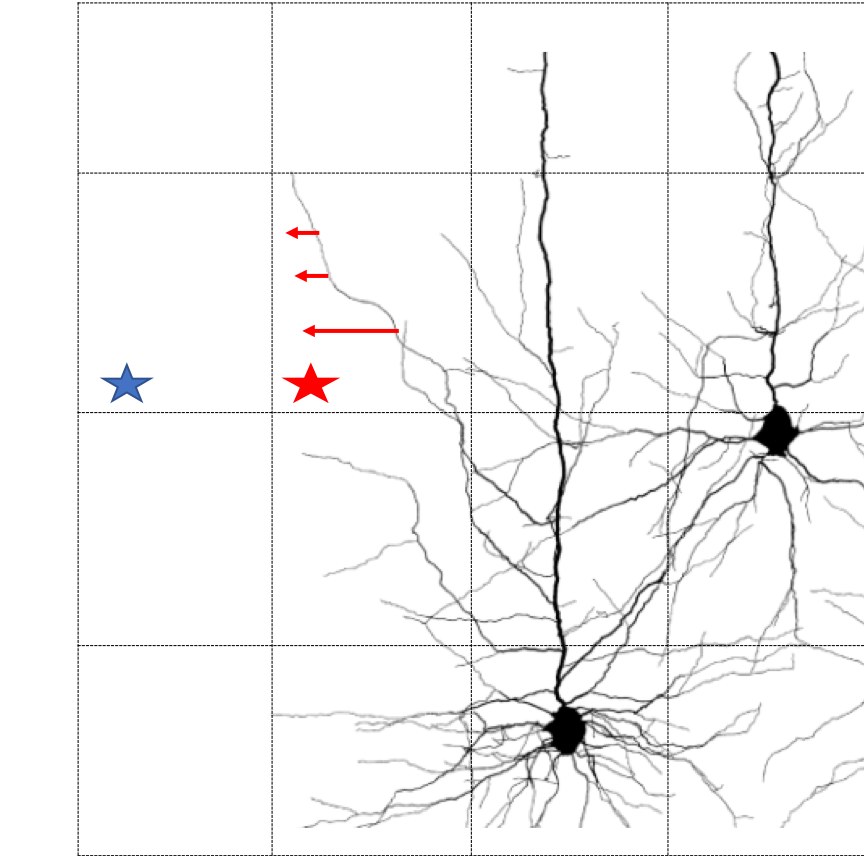
\includegraphics[width=0.5\textwidth]{Figures/KNP.png}
\end{center}
\caption{\textbf{KNP scheme}. Blue star: Mesh cell containing no neuronal sources, so that $C=0$. Red star: Mesh cell containing neural sources. Here $C$ can be computed by summing over all neuronal transmembrane currents, including the capacitive current, and dividing by the volume of the mesh cell. LAGE LITT MER INFORMATIV FIG HER OM VI SKAL HA FIG HER.}
\label{fig:KNPmesh}
\end{figure}


\subsection{Do diffusion potentials matter?}
Due to the computational challenges they impose, it is tempting to make the assumption that diffusive currents contribute so little to the extracellular potential that we don't have to bother with them. This is what normally is being done, as most theoretical studies of extracellular potentials are based on standard VC theory. For most purposes, this is probably a good approximation, but its validity depends on one of the two following criteria being met:

\begin{enumerate}
\item C1: The magnitude of diffusive currents is much smaller than the magnitude of Ohmic drift currents.
\item C2: The frequency of diffusive currents is much smaller than the frequency of the CSD and the Ohmic drift currents. 
\end{enumerate}

The first criterion is general and quite intuitive. If C1 holds, the last term in eq. \ref{eq:eldiffCSD2} becomes much smaller than the other two terms, and standard VC theory will give accurate predictions of $\phi$. As we shall see below, it is quite likely that C1 is violated under many physiological conditions. If so, the second criterion (C2) may still come to our rescue, as in most experiments, extracellular potentials are recorded using electrode systems with a lower cut-off frequency of 0.1-1 Hz \cite{Einevoll2007}. As diffusive currents are proportional to concentration gradients, which generally vary at a much slower time scale than $\phi$, diffusive contributions to $\phi$ are often direct-current (DC) like, i.e., almost constant in time. If so, they will not be picked up in recordings using standard electrode systems, only in experiments using DC electrodes. The question regarding their contribution to standard measurements is then whether they are DC-like enough. 

In the two following sub-sections we shall explore when and to which degree the criteria C1-C2 are likely to be met under physiological conditions.

\subsubsection{Magnitude of diffusion potentials.}
Here, we will make some crude estimation of the magnitude that we can expect diffusion potentials to have in neural tissue. To make these, make the following simplifications of eq. \ref{eq:eldiffCSD2}): Firstly, diffusion potentials depend solely on extracellular concentration gradients, and not on the instantaneous activity of neurons. Let us therefore assume that $CSD = 0$, and consider the extracellular dynamics is governed by
\begin{equation}
\nabla \cdot (\sigma_e\nabla\phi_d) = - \nabla \cdot \left (\sum_k{F z_k \tilde{D_k}{\bf \nabla} c_{k}} \right), 
\label{eq:eldiffCSD3}
\end{equation}
where we have denoted the potential $\phi_d$ since, in this case, it will exclusively be evoked by diffusion. Let us further consider a system with closed boundaries, so that no current can enter/leave the system. In that case, we may simply skip the first nabla, and take:
\begin{equation}
\sigma_e\nabla\phi_d = -\sum_k{F z_k \tilde{D_k}{\bf \nabla} c_{k}}, 
\label{eq:diffpot}
\end{equation}
Essentially, eq. \ref{eq:diffpot} states that the Ohmic drift current and diffusive current must cancel each others at each point in space, i.e., that if no current enters the system from the outside, no net current should be observed anywhere inside the system. The diffusion potential is thus the potential that we must have in the system for this to be the case. 

Finally, due to the linearity in eq. \ref{eq:diffpot}, the diffusion potential between two points in space is a direct function of the the ionic concentrations at these two points. Hence, it is sufficient for our task to consider a simple two-compartment system (like that in Fig. \ref{fig:diffpot}). For two-compartment systems, eq. \ref{eq:diffpot} further simplifies to:

\begin{equation}
\Delta \phi_d = \frac{F}{\bar{\sigma_e}} \sum_k{z_k \tilde{D}_k \Delta c_k}
\label{eq:diffpot2}
\end{equation}
where $\Delta c_k = c_{k}^{2} - c_{k}^{1}$ and $Delta \phi_d = \phi_d^{2} - \phi_d^{1}$ denote the concentration and potential difference between compartments 1 and 2. Within each compartment, $\sigma_e$ can be determined from the ionic concentrations by use of eq. \ref{eq:sigma1}. However, since we for this problem need the conductivity experienced by an Ohmic current traveling between the two compartments, we have in eq. \ref{eq:diffpot2} used the average $\sigma_e$ of the two compartments:
\begin{equation}
\sigma_e = \frac{F}{2\psi}\sum_{k} \left(\tilde{D}_k z_{k}^2 c_{k}^{1} + \tilde{D}_k z_{k}^2 c_{k}^{2} \right).
\label{eq:sigma2}
\end{equation}

Based on eq. \ref{eq:diffpot2}, we make some estimates of the magnitude of the diffusion potential for some test examples.

\begin{itemize}

\item {\bf Diffusion potential under spreading depression:} The most extreme extracellular concentration shifts in the brain occur under the pathological condition called spreading depression, where the extracellular K$^+$ concentration can change by several tens of millomolars. In an an example from hippocampus, the K$^+$ concentration was about 30 mM higher at the bottom hippocampal layer than at the top hippocampal layer (Fig. 1a in \cite{Herreras1993}). In that experiment, only K$^+$ concentrations were recorded. However, we may give a crude estimate of the diffusion potential between the top and bottom of hippocampus by making some simple assumptions of the other ion concentrations: (i) We assume that the top layer of hippocampus remained at baseline concentrations. In the experiment, this seemed to be close to the case for $c_K$ \cite{Herreras1993}. In the top layer, we may therefore assume some rather typical baseline concentrations with $c_{Na} = 150$ mM, $c_{K} = 3$ mM and $c_{Cl} = 153$ mM. (ii) In the bottom layer, we assume that the $c_K$ was 30 mM above baseline, and that the increase in $c_K$ was compensated by an identical decrease in $c_{Na}$, so that electroneutrality was preserved. A plausible mechanism behind this would be that all concentration shifts were due to neuronal AP firing, i.e., neurons exchanging Na$^+$ for K$^+$. With these assumptions, we have $c_{Na} = 120$ mM, $c_{K} = 33$ mM and $c_{Cl} = 153$ mM in the bottom layer. Plugging the top layer and bottom layer co ncentrations into eq. \ref{eq:diffpot2}, we obtain a diffusion potential $\Delta \phi_d \sim 1$ mV across the hippocampal depth.

\item {\bf Diffusion potential in cortex during neuronal hyperactivity:} In several experimental papers, extracellular concentration shifts of selected ions have been recorded during induced neuronal hyperactivity and seizure activity \cite{kriv1975, nicholson1978, Dietzel1982, somjen1986, Dietzel1989}. The main focus of these works are typically on $c_K$, which is the most critical extracellular concentration due to its low baseline value. In these experiments, $c_K$ can typically change from a baseline value around 3 mM up to a ceiling level between 8-12 mM before the dynamics becomes pathological and is driven into spreading depression. Dietzel et al. estimated the concentration shifts in both $c_{K}$, $c_{Na}$ and $c_{Cl}$, and cased on a series of recordings, they estimated that the maximal diffusion potential that could be expected under their experimental condition was 0.4 mV \cite{Dietzel1989}.

\item{\bf Diffusion potential during normal activity:} It is difficult to find experimental data that allows us to estimate diffusion potentials in the brain under "normal" conditions, and the question as to whether concentration gradients are present in a given brain region probably depends on the processing state it is in. However, recordings from anesthetized cat cortex have shown that even during the resting state, $c_K$ may exhibit small-amplitude (0.5 mM) fluctuations \cite{MCCREERY1983}. In experiments recording the response in cortex to moderate (not seizure inducing) stimuli applied in the thalamus, cortical $c_K$ increases were found to have a depth profile, and vary by about 2 mM between different cortical layers \cite{Cordingley1978}. Thus, it seems likely that there should be some concentration gradients present in neural systems, and that e.g., a concentration difference of about 1 mM between the top and bottom of cortex or hippocampus would not be unlikely under normal processing. If we repeat the calculation from spreading depression, but assume that $c_{K}$ and $c_{Na}$ in the bottom layer were increased/decreased by 1 mM instead of 30 mM, we get a diffusion potential of about $33 \mu$V. This is of the same magnitude as potentials typically recorded in LFP recordings. 

\end{itemize}

Based on the above estimates, diffusion potentials can not as a generality be expected to be so small that they can be ruled out as possible contributors to the LFP. 


\subsubsection{Frequency of diffusion potentials}
\ghnote{Krevende kapittel. Sammenligne noen powerspectra her. Regne ut et par selv, ala Gratiy.} 

Previous computational studies have predicted that effects of diffusion on extracellular potentials are not necessarily small, but tend to be very slow, meaning that they will only affect the very low-frequency components of $\phi$ \citep{Halnes2016, Halnes2017}. This is due to the diffusive current being a direct function of ion concentrations $c_k$, which on a large spatial scale typically vary on a much slower time scale (seconds-minutes) than the fluctuations in $\phi$ that we commonly are interested in (milliseconds-seconds). Furthermore, electrodes used to record $\phi$ typically have a lower cutoff frequency of 0.1-1Hz \citep{Einevoll2013}, which means that most of the tentative diffusive contribution will be filtered out from experimental recordings. It may therefore be a good approximation to neglect the diffusive term, except in the case of pathologically dramatic concentration variations.
